% =============================================================================
%  s02_desarrollo.tex — Sección 2: Desarrollo / Argumentación central
%  Agrega tantos frames como necesites dentro de cada subsección.
% =============================================================================

\section{Marco Conceptual y Análisis}


% --- Diapositiva 2.1 y 2.2: Crisis de Expansión y Motorización ---
\begin{frame}{La Crisis de la Expansión y Motorización en México}
    \begin{columns}[T]
        \begin{column}{0.5\textwidth}
            \begin{block}{Expansión vs. Población}
                De acuerdo con datos de SEDESOL, las ciudades mexicanas han crecido físicamente a tasas desproporcionadas \cite{SEDESOL2012}:
                \begin{itemize}
                    \item \textbf{Superficie:} Incremento de \textbf{6 veces}.
                    \item \textbf{Población:} Incremento de solo \textbf{1.9 veces}.
                \end{itemize}
                \textbf{\small Este modelo disperso genera ineficiencia energética y segregación \cite{ITDP_Espacio}.}
            \end{block}
        \end{column}
        \begin{column}{0.5\textwidth}
            \begin{alertblock}{Fenómeno de Motorización}
                Según el IMCO, el parque vehicular crece a una tasa anual del \textbf{5.3\%}, lo que representa un ritmo \textbf{3.5 veces más rápido} 
                que el crecimiento poblacional (1.5\%) \cite{IMCO2019Doc}. \\
                \textbf{\small El transporte es actualmente el sector de mayor consumo energético nacional \cite{ITDP_Espacio}.}
              \end{alertblock}
        \end{column}
    \end{columns}
\end{frame}

% --- Diapositiva: Modelos de Densificación (Solicitada) ---
\begin{frame}{Modelos de Densificación Evaluados}
  \begin{columns}[T]
    \begin{column}{0.32\textwidth}
      \begin{block}{Modelo 1: TOD}
        \textbf{\textit{Transit-Oriented\\Development}\\[0.2cm]}
        ¿Dónde se implementó? Copenhague, Estocolmo\\[0.1cm]
        {\small Principio: compacidad alrededor de nodos de transporte masivo \cite{ITDP_Espacio}.}
      \end{block}
    \end{column}
    \begin{column}{0.32\textwidth}
      \begin{block}{Modelo 2: Barrio}
        \textbf{\textit{Rehabilitación\\incremental}\\[0.2cm]}
        ¿Dónde se implementó? Medellín, Bogotá\\[0.1cm]
        {\small Principio: participación comunitaria y urbanismo social.}
      \end{block}
    \end{column}
    \begin{column}{0.32\textwidth}
      \begin{block}{Modelo 3: Corredor}
        \textbf{\textit{Corredor\\urbano mixto}\\[0.2cm]}
        ¿Dónde se implementó? Ciudad de México\\[0.1cm]
        {\small Principio: mixticidad de usos sobre ejes de movilidad masiva.}
      \end{block}
    \end{column}
  \end{columns}
\end{frame}

% ── Frame: Reporte 00 - Logs de Ejecución ────────────────────────────────────
\begin{frame}[fragile]{Reporte 00: Ejecución Algorítmica y Consolidación}
  \begin{block}{Logs de Construcción del Grafo (VFT\_Model)}
    \fontsize{7pt}{8pt}\selectfont
    \begin{verbatim}
      2026-04-18 20:46:41 | INFO | Fase 1 y 2: Extrayendo nodos y trazos base...
      2026-04-18 20:46:43 | INFO | Fase 2 completada: 65220 aristas creadas.
      2026-04-18 20:46:43 | INFO | Grafo Base: 11115 Nodos y 32344 Segmentos.
      2026-04-18 20:46:43 | WARN | Eliminadas 1562 aristas phantom (> 5 km).
      2026-04-18 20:46:43 | INFO | Fase 3: Integrando sistemas (Tolerancia: 85.0m)...
      2026-04-18 20:47:09 | INFO | Se crearon 20482 aristas de Transbordo Peatonal.
      2026-04-18 20:47:09 | INFO | Impedancia aplicada exitosamente a 25197 segmentos.
      2026-04-18 20:47:09 | INFO | Grafo final: 11115 nodos, 45679 aristas.
    \end{verbatim}
  \end{block}

  \begin{columns}[T]
    \begin{column}{0.48\textwidth}
      \begin{exampleblock}{Eficiencia de Reducción}
        Se logró una reducción del \textbf{~90\%} de la inflación topológica, consolidando una red operativa de \textbf{11,115 nodos} \cite{Garibaldi2024VFT}.
      \end{exampleblock}
    \end{column}
    \begin{column}{0.48\textwidth}
      \begin{itemize}
        \item \textbf{Aristas de Transporte:} 25,197 segmentos procesados con impedancia real.
        \item \textbf{Conectividad:} Integración exitosa de transbordos intermodales.
      \end{itemize}
    \end{column}
  \end{columns}
\end{frame}

% ── Frame: Reporte 00 - Snapping Lógico y Resultados ─────────────────────────
\begin{frame}{Resultados del Análisis Espacial: Snapping Lógico}
  \begin{columns}[T]
    \begin{column}{0.55\textwidth}
      \centering
      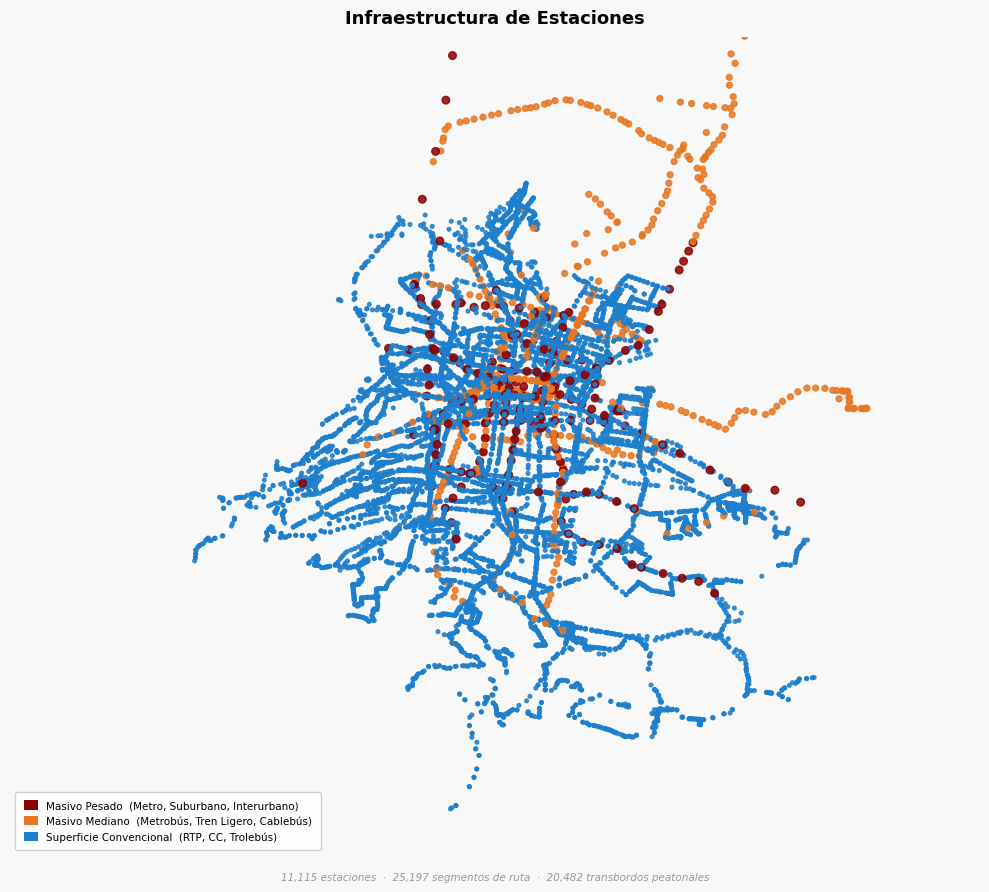
\includegraphics[width=\textwidth, height=5.5cm, keepaspectratio]{img/grafica_infraestructura.png}
      \fuentefigura{Elaboración propia basada en datos de Apimetro y Modelo VFT \cite{Garibaldi2024VFT}.}
    \end{column}

    \begin{column}{0.42\textwidth}
      \begin{itemize}
        \item \textbf{Fundamentación Metodológica:} El uso de \textit{Apimetro} alinea la investigación con las 
              tendencias de Ciencia de Datos en Urbanismo \cite{ramirez2025analisis}.
        \item \textbf{Resolución de Inflación:} El uso de \texttt{KDTree} responde a la crítica de grafos ruidosos 
                para asegurar cálculos de accesibilidad veraces \cite{Garibaldi2024VFT}.
      \end{itemize}
    \end{column}
  \end{columns}
\end{frame}

% --------- Frame de Alineación --------
\begin{frame}{Lineamientos de Política Pública}
  \begin{enumerate}
        \item \textbf{Fundamentación Metodológica:} Al utilizar el proyecto de código abierto Apimetro, la investigación 
        se alinea con las tendencias actuales de Ciencia de Datos aplicada al Urbanismo \cite{ramirez2025analisis}.
        \item \textbf{Resolución de la Inflación Topológica:} El uso del \texttt{scipy.spatial.KDTree} no es solo una elección técnica, 
        sino una respuesta a la crítica de los grafos teóricos ruidosos \cite{ramirez2025analisis}.
        \item \textbf{Impacto en la Política Pública:} Al asegurar la continuidad operativa, el Modelo VFT permite pasar de una 
        planeación teórica a una basada en conectividad operativa real, lo cual es un requisito indispensable para alcanzar las 
        metas de accesibilidad y eficiencia que dicta \cite{SEDATU2023}.
  \end{enumerate}
\end{frame}



% ── Frame: Solo texto — mensaje clave, cita o puente entre secciones ─────────
%    USO: para declaraciones fuertes, preguntas retóricas o transiciones.
%    Copia y adapta. No lleva título de frame ni elementos gráficos.
\begin{frame}[plain]
  \begin{tikzpicture}[remember picture, overlay]
    % Banda lateral de color
    \fill[ColorPrincipal]
      (current page.north west) rectangle
      ([xshift=0.35cm] current page.south west);
    % Línea dorada en el borde de la banda
    \fill[ColorAcento]
      ([xshift=0.32cm] current page.north west) rectangle
      ([xshift=0.35cm] current page.south west);
  \end{tikzpicture}
  \hspace{0.8cm}%
  \begin{minipage}{0.88\textwidth}
    \vspace{2.2cm}
    {\color{ColorAcento}\rule{0.5\textwidth}{1.2pt}}\\[0.5cm]
    {\large\bfseries\color{ColorPrincipal}
      ¿Puede la infraestructura de movilidad\\
      actuar como frontera ecológica?}\\[0.6cm]
    {\normalsize\color{black}
      Una intervención de transporte masivo bien diseñada no destruye
      el territorio: lo delimita, lo protege y lo articula.}\\[0.5cm]
    {\color{ColorAcento}\rule{0.3\textwidth}{0.8pt}}
    \vfill
  \end{minipage}
\end{frame}
